Dans un repère orthogonal, donnons nous la parabole $\geoset{P} : y = x^2$ . Plaçons-y les points $A$ , $B$ et $S$ d'abscisses respectives $a$ , $b$ et  $s = a + b$ .
Observez
\footnote{
	Le lieu de téléchargement de ce document contient un fichier GeoGebra \texttt{base-tool.ggb} manipulable dynamiquement pour vérifier combien il est aisé de conjecturer quelque chose.
}
les trois cas ci-dessous et essayez de conjecturer quelque chose \emph{(la réponse est donnée dans la page suivante)}.


\vspace{2.5em}

\begin{multicols}{2}
	\center
	\footnotesize
	\itshape
	
	\fbox{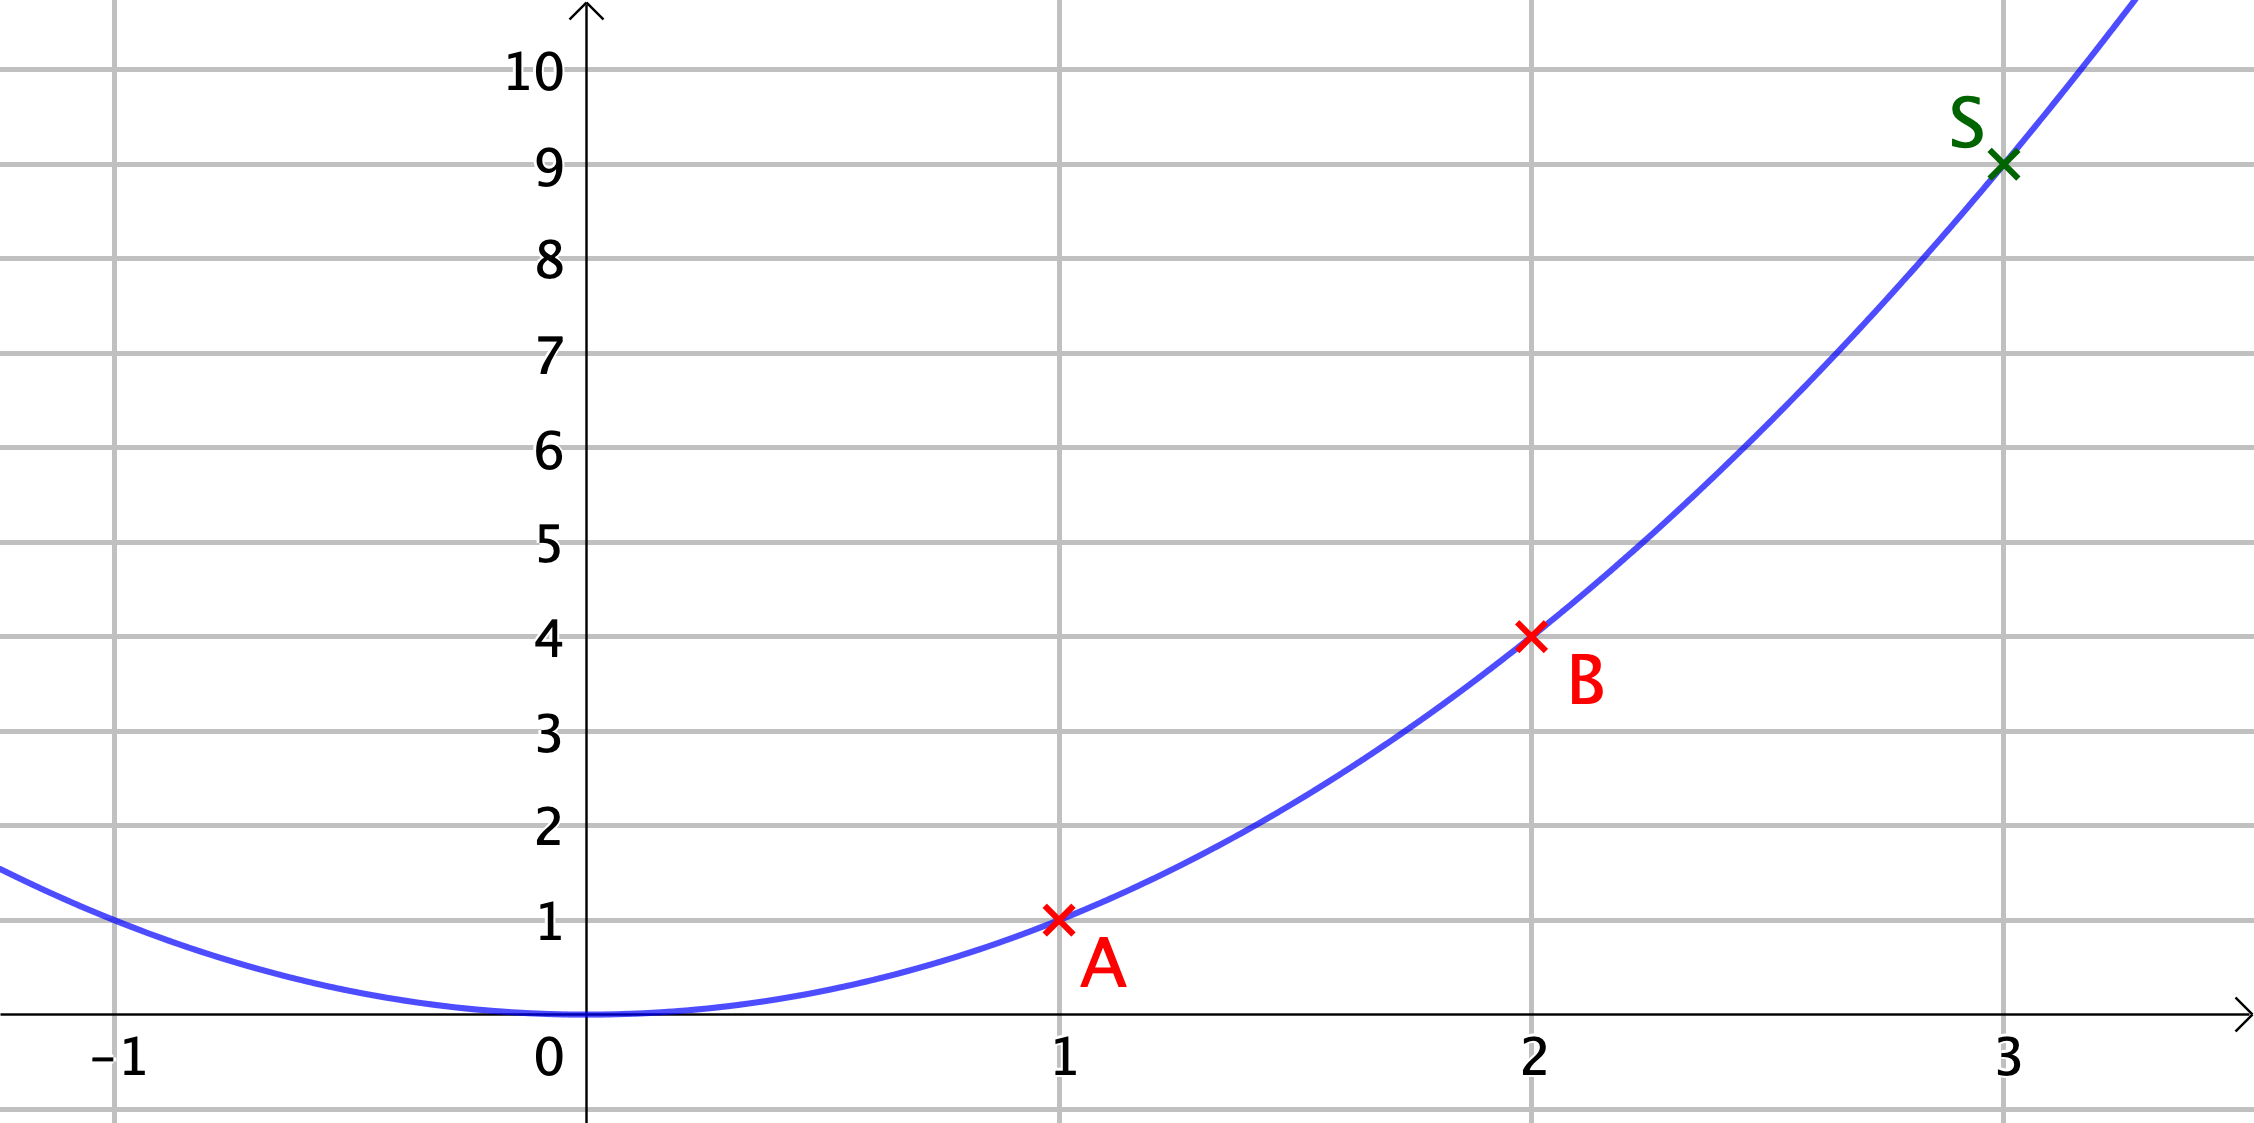
\includegraphics[scale = .8]{addition-on-parabolas/conjecture/a-and-b-positive.png}}
	
	\smallskip
	Cas où $a > 0$ et $b > 0$

	\columnbreak
	
	\fbox{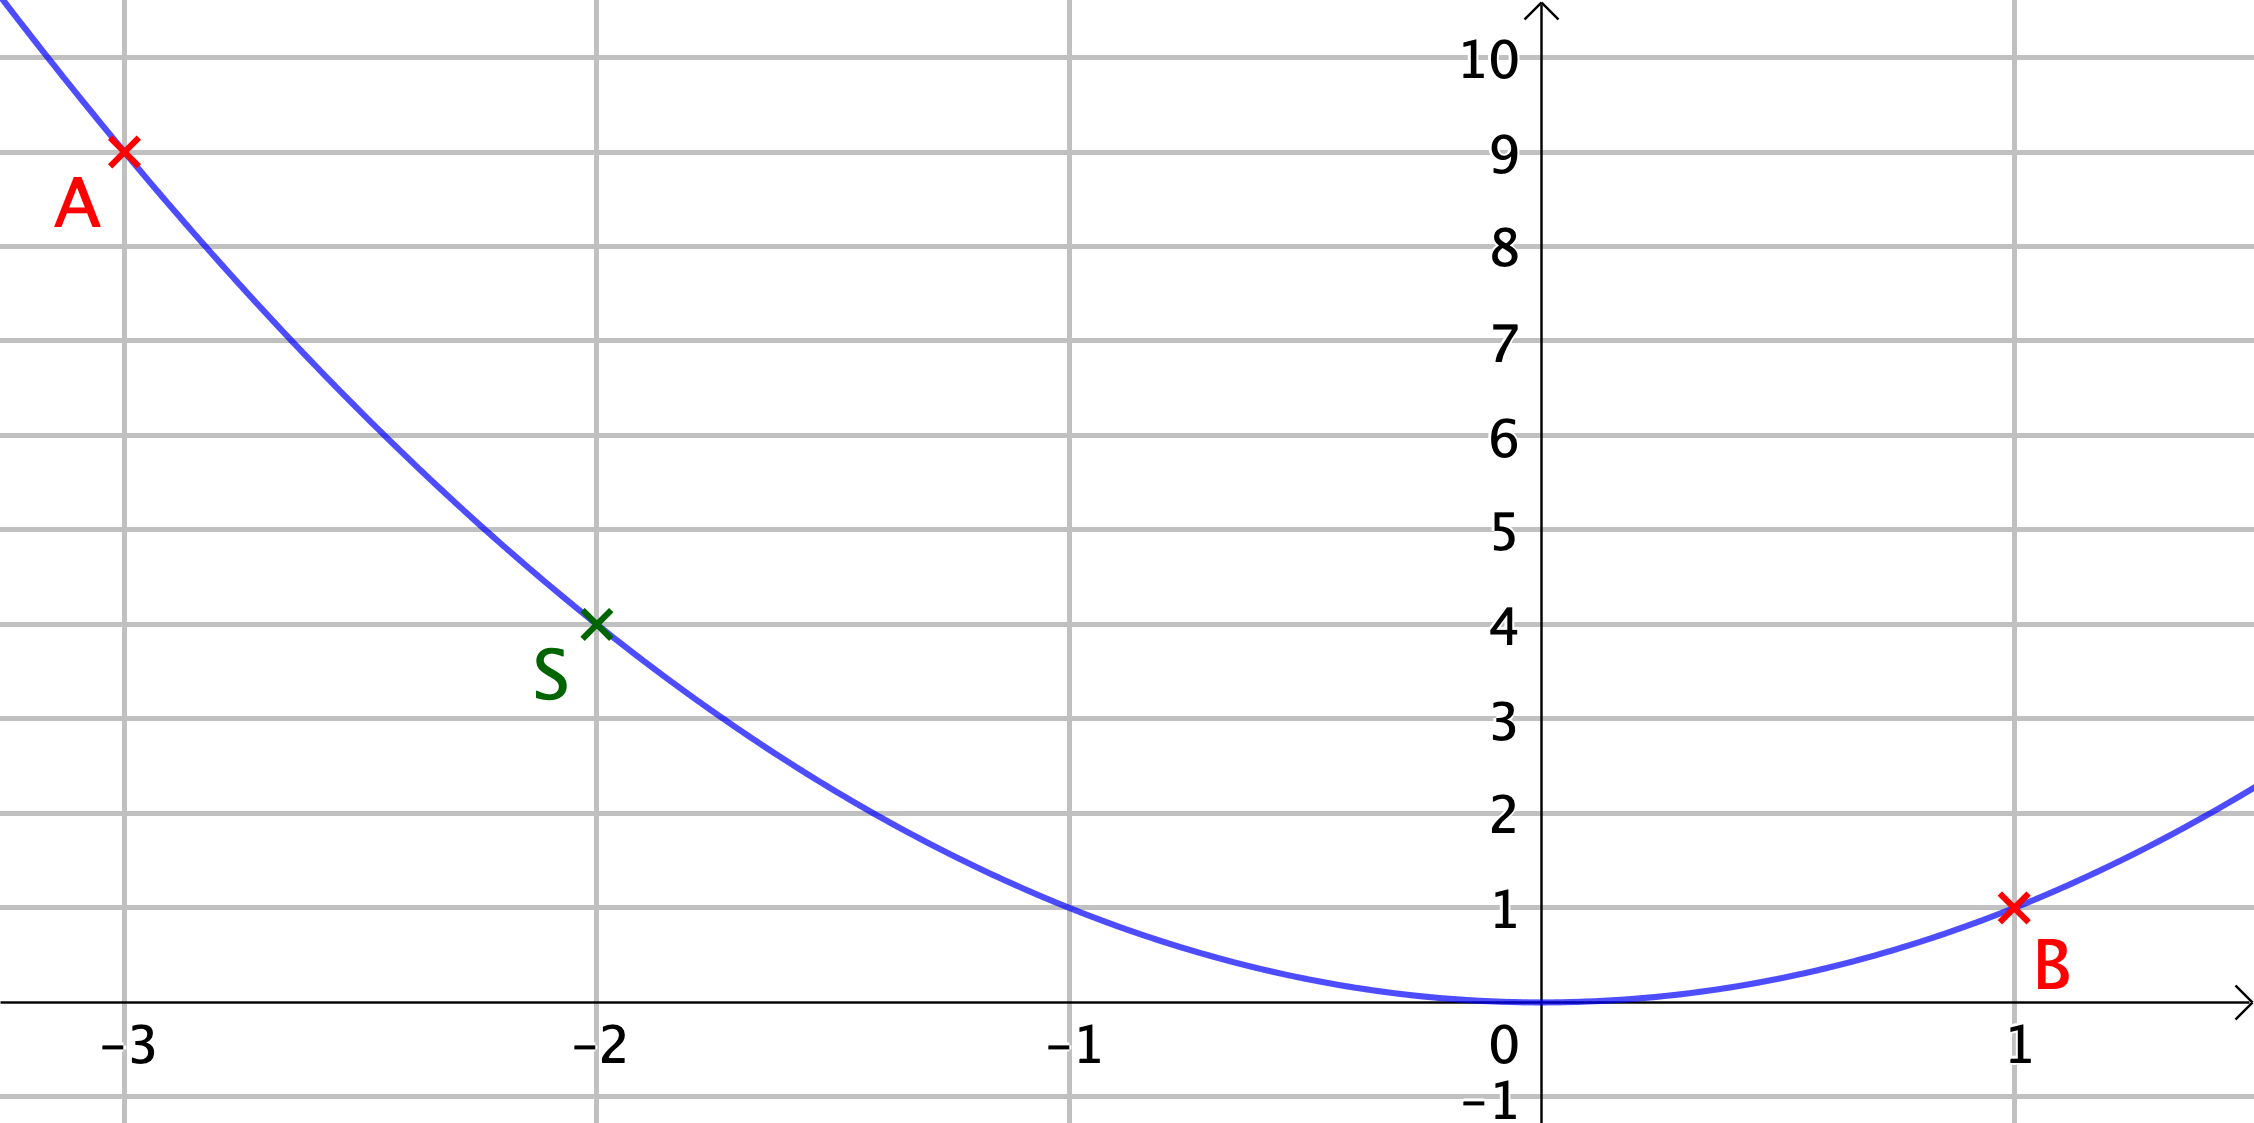
\includegraphics[scale = .8]{addition-on-parabolas/conjecture/a-and-b-diff-signs.png}}
	
	\smallskip
	Cas où $a < 0$ et $b > 0$
\end{multicols}
	
\begin{center}
	\footnotesize
	\itshape

	\fbox{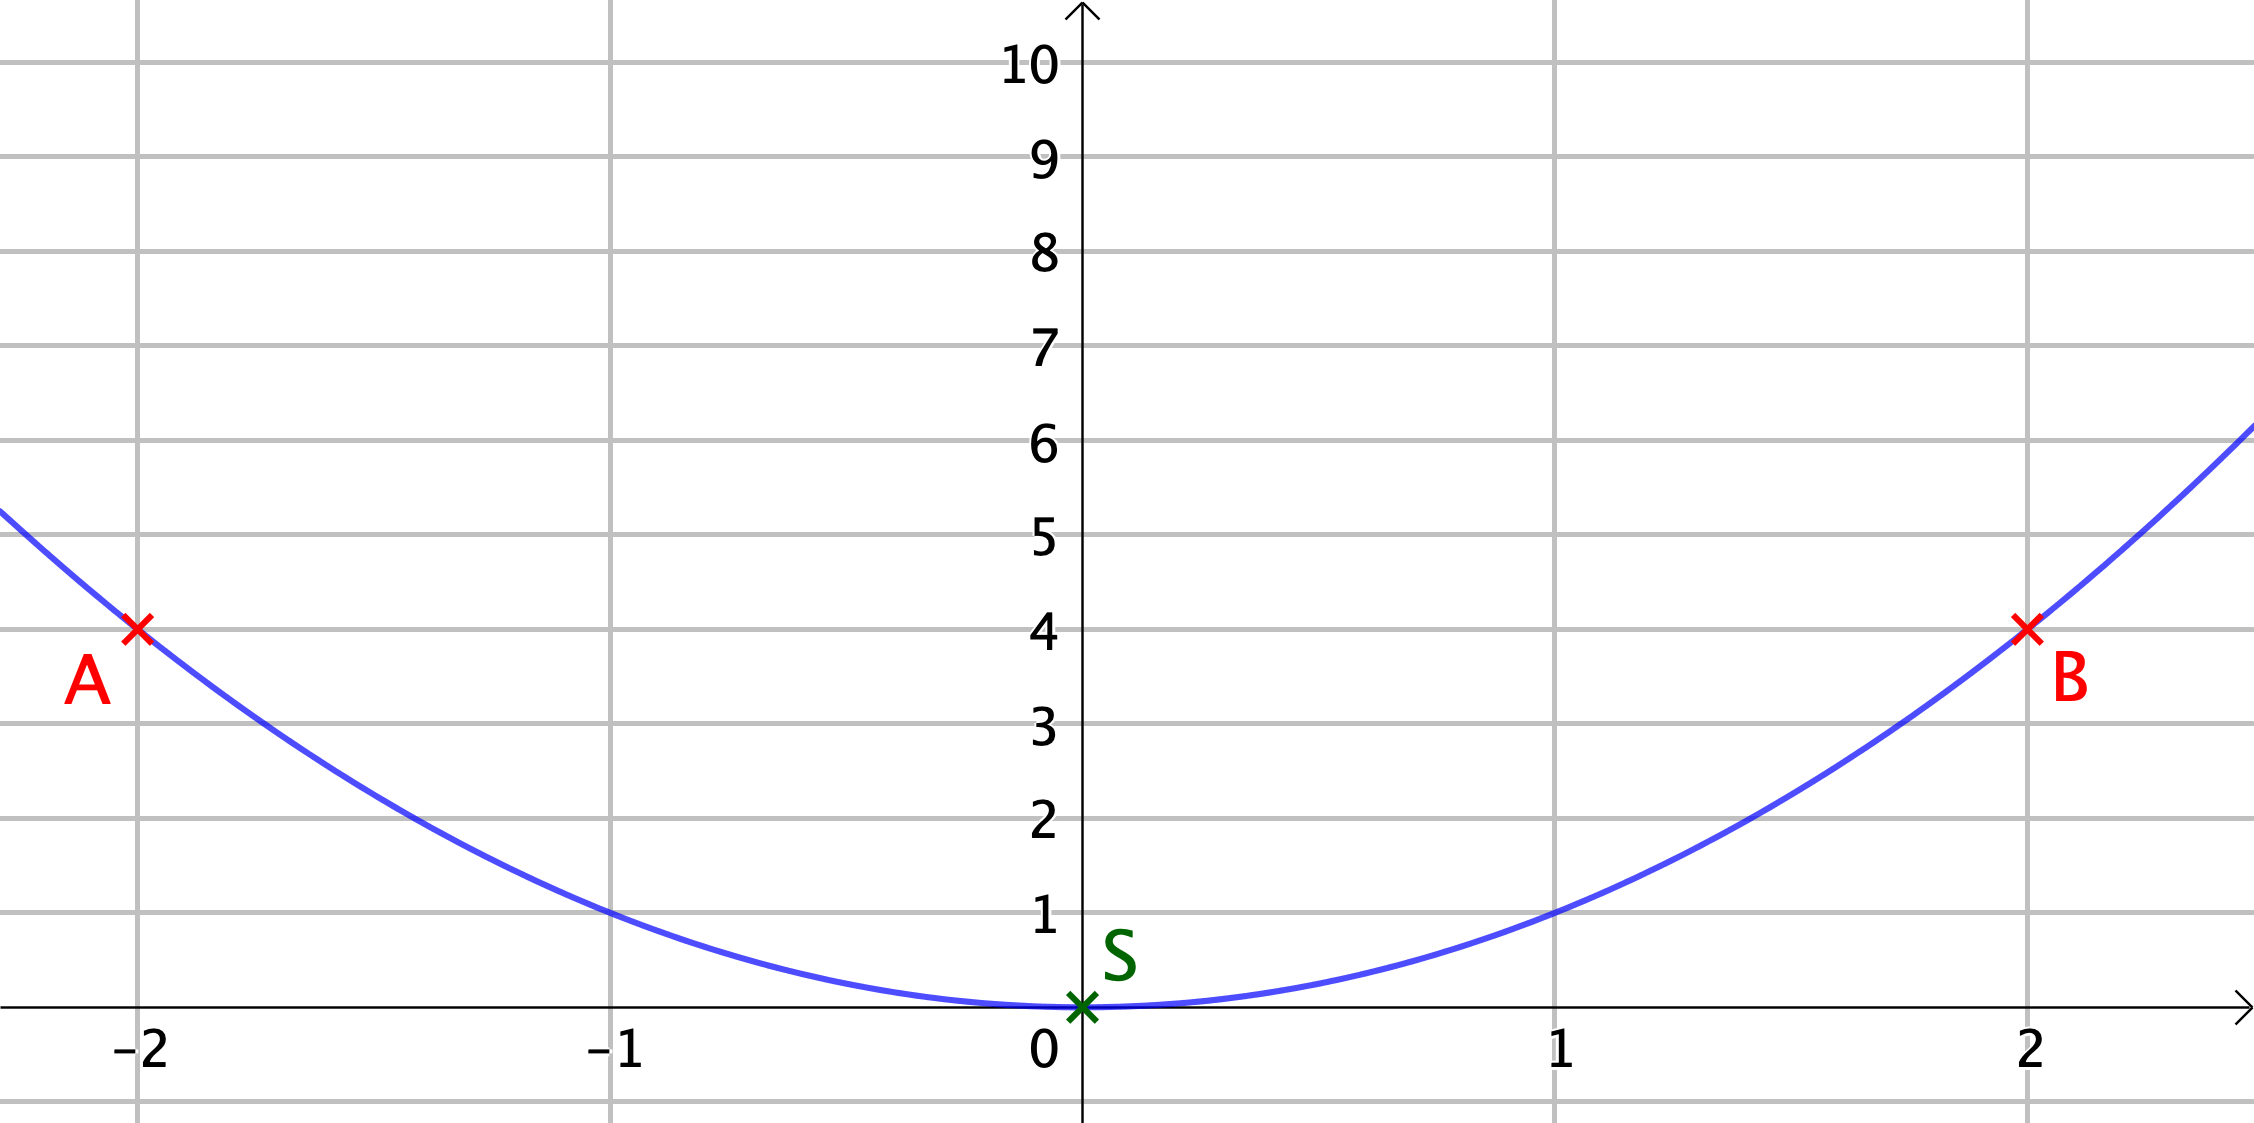
\includegraphics[scale = .8]{addition-on-parabolas/conjecture/a-and-b-opposite.png}}
	
	\smallskip
	Cas où $a = -b$
\end{center}


\newpage

Pour mieux voir ce qu'il se passe, traçons quelques droites. Voici ce que cela donne.

\begin{multicols}{2}
	\center
	\footnotesize
	\itshape

	\fbox{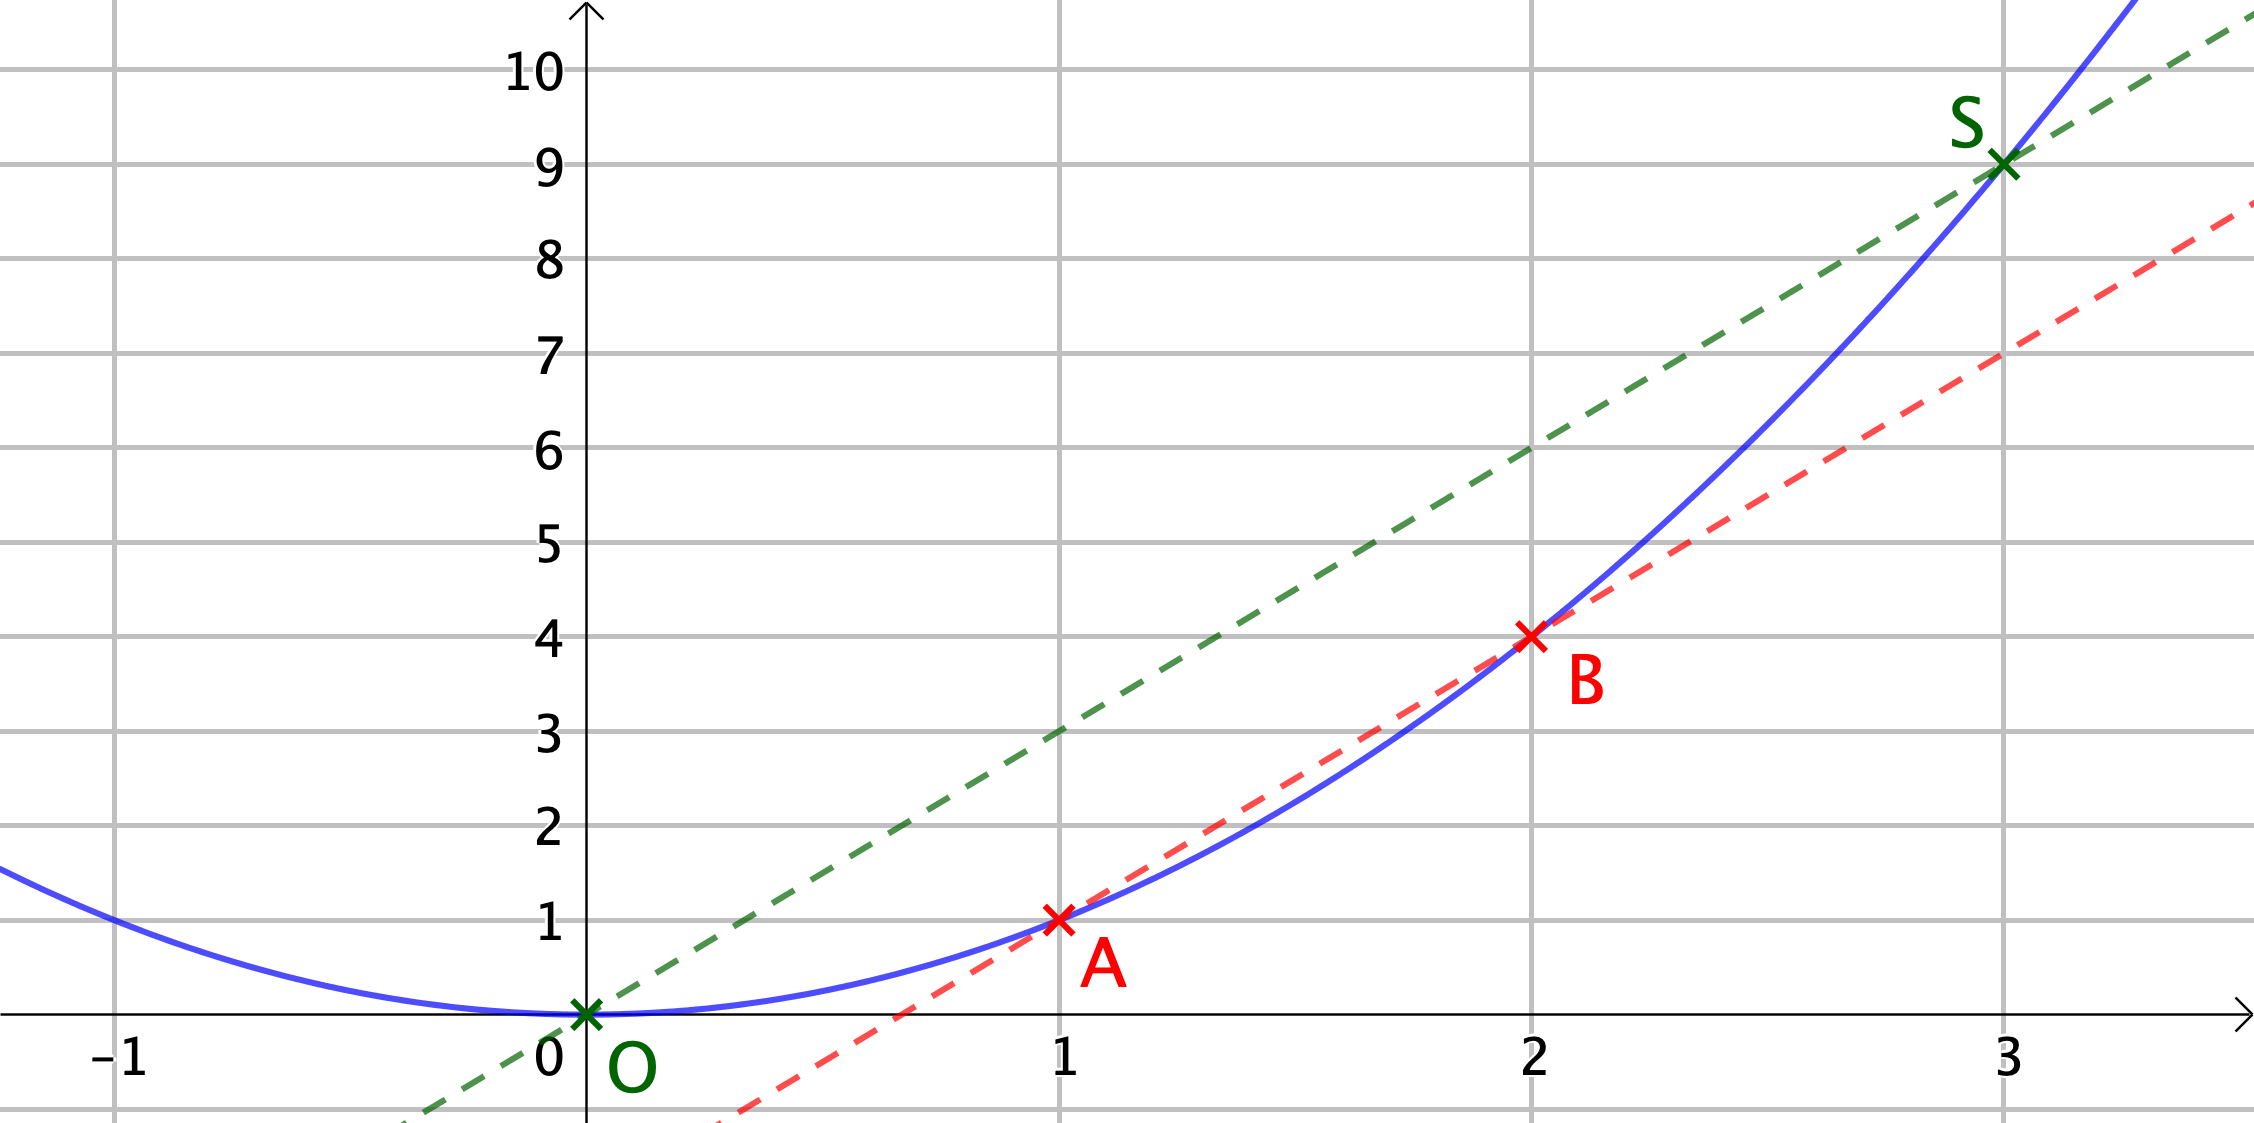
\includegraphics[scale = .8]{addition-on-parabolas/conjecture/a-and-b-positive-with-lines.png}}
	
	\smallskip
	Cas où $a > 0$ et $b > 0$

	\columnbreak
	
	\fbox{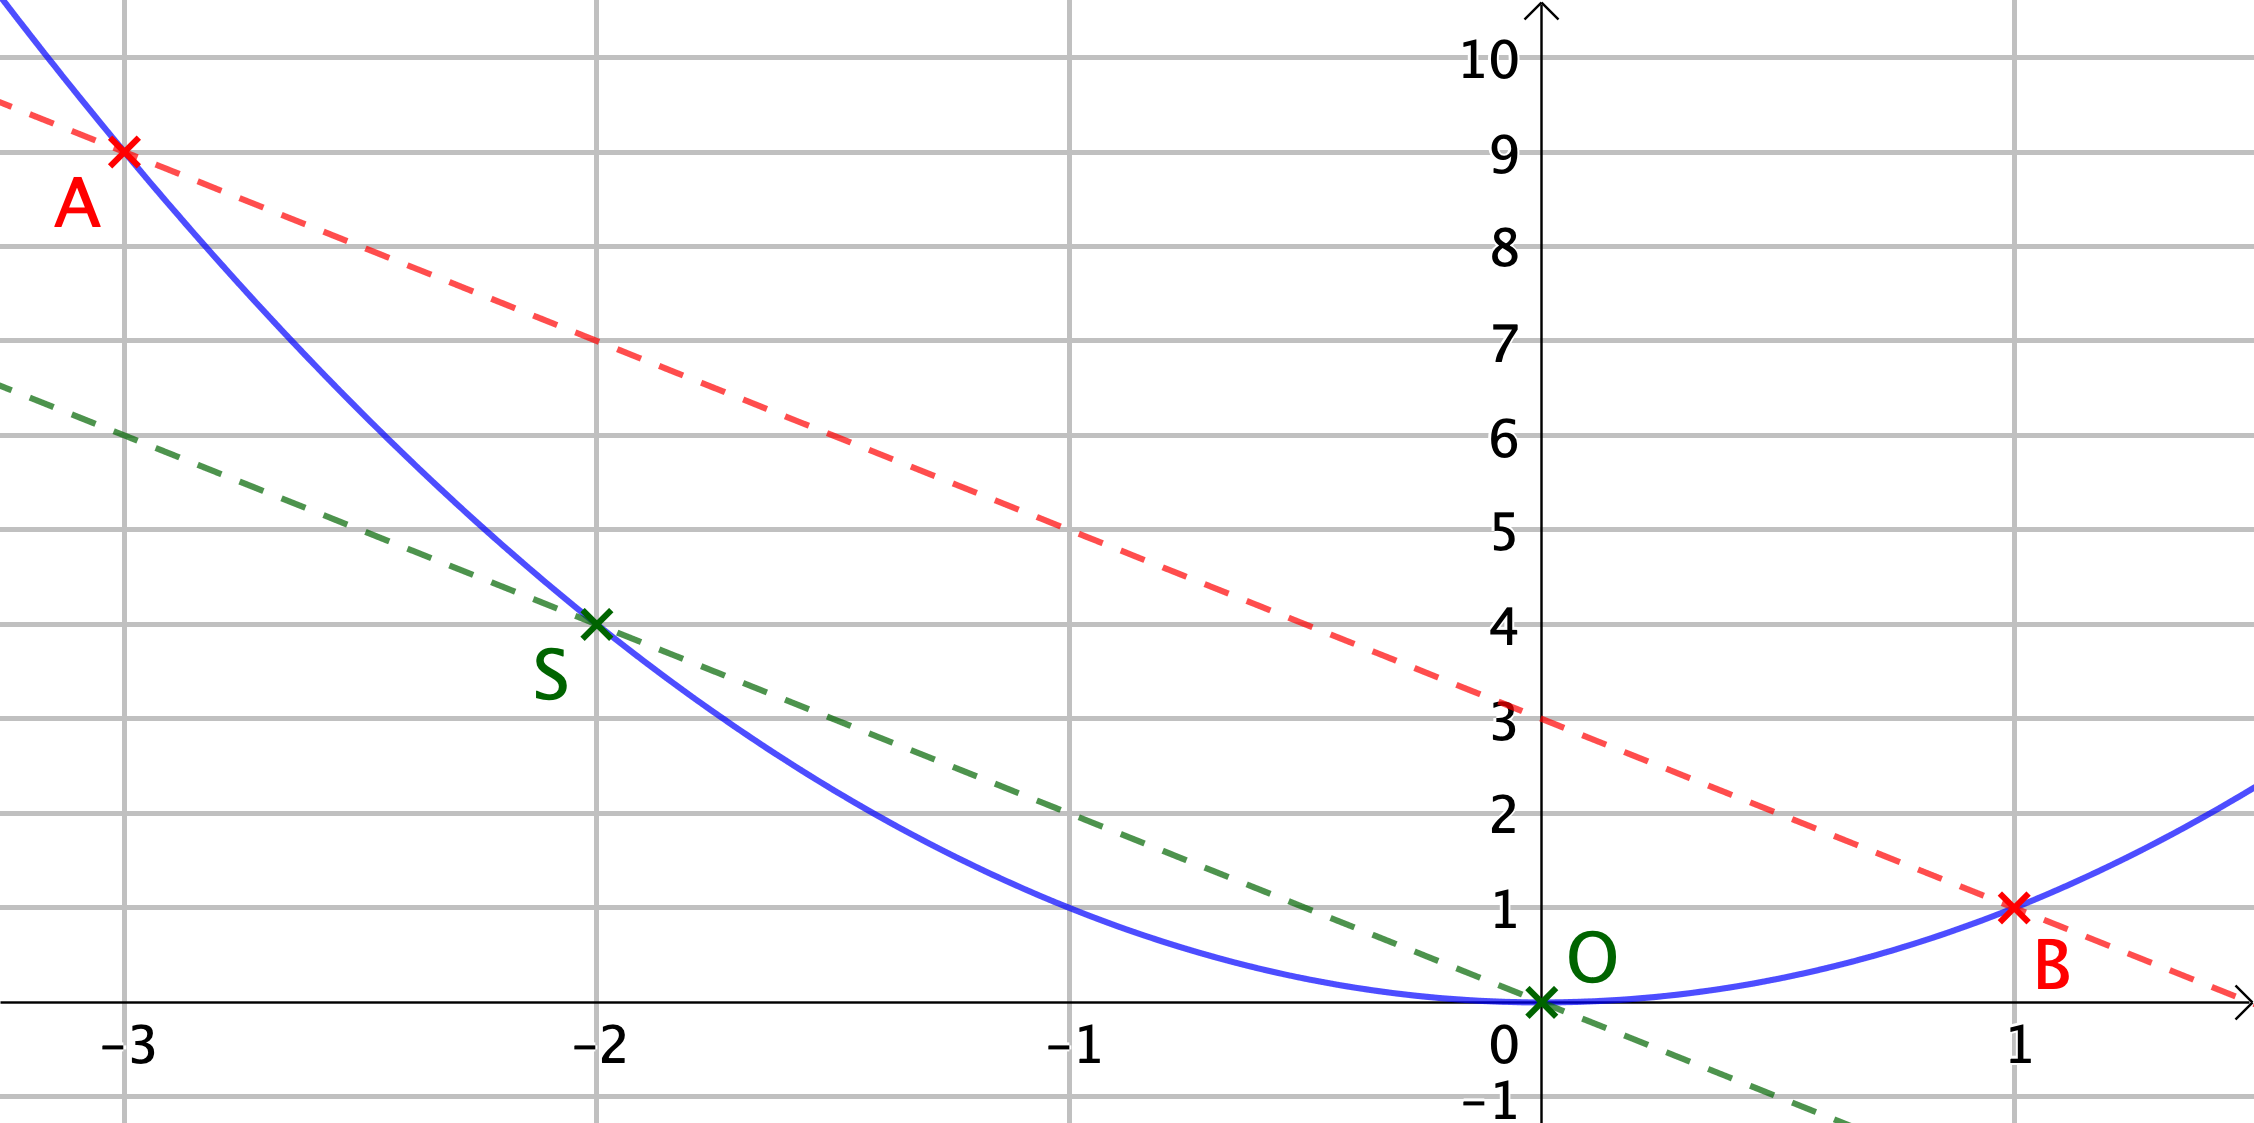
\includegraphics[scale = .8]{addition-on-parabolas/conjecture/a-and-b-diff-signs-with-lines.png}}
	
	\smallskip
	Cas où $a < 0$ et $b > 0$
\end{multicols}
	
\begin{center}
	\footnotesize
	\itshape

	\fbox{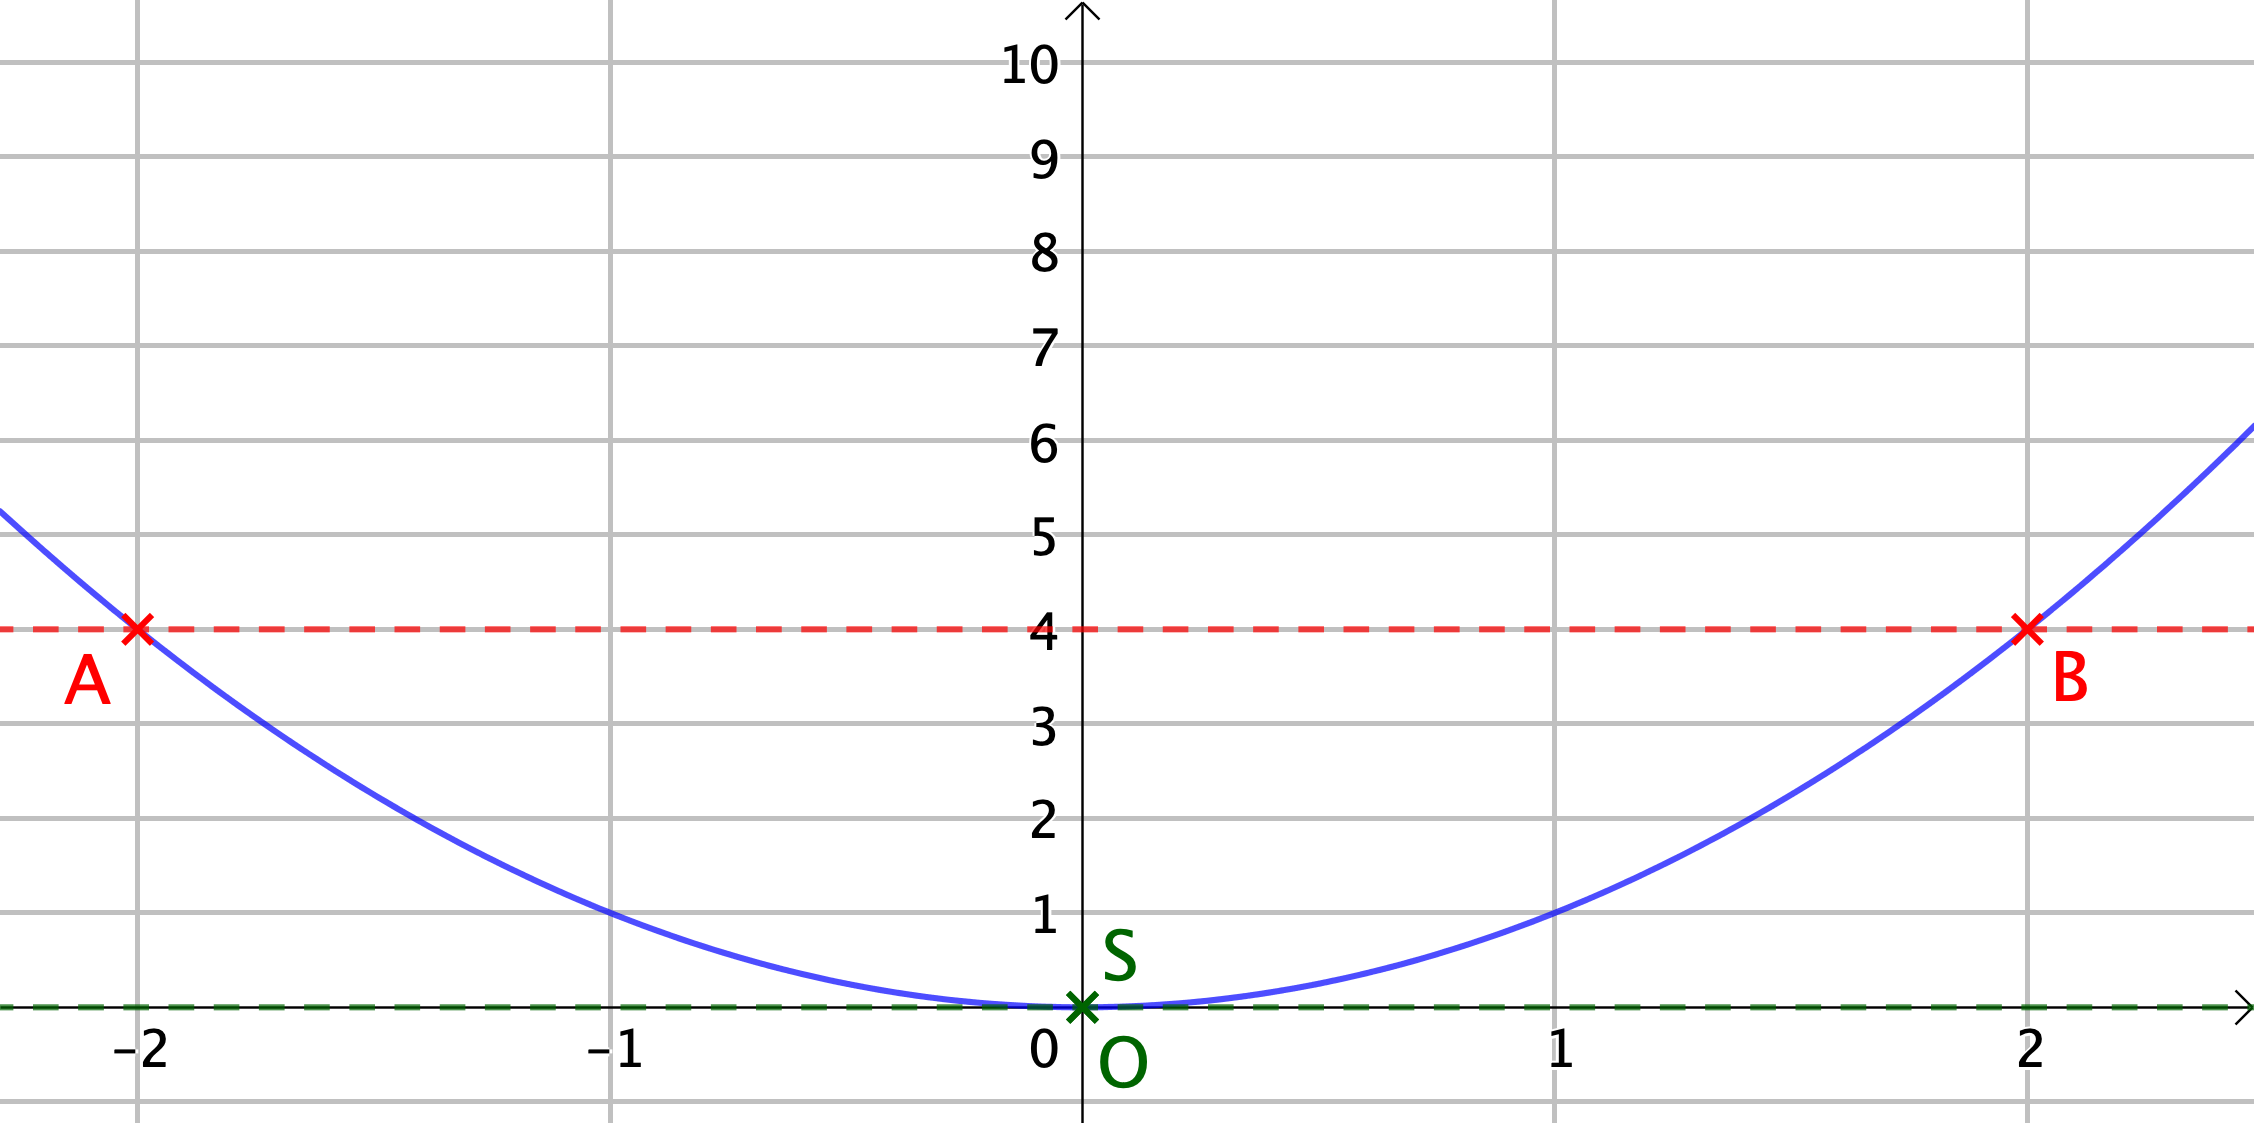
\includegraphics[scale = .8]{addition-on-parabolas/conjecture/a-and-b-opposite-with-lines.png}}
	
	\smallskip
	Cas où $a = -b$
\end{center}


\medskip

Il devient évident de conjecturer que le point $S$ se construit géométriquement comme suit.

\begin{enumerate}
	\item \label{point-1} Si $x_A \neq \pm \, x_B$ alors on construit la parallèle à $(AB)$ passant par $O$ l'origine du repère. Le point $S$ est le second point d'intersection de cette parallèle avec $\geoset{P}$  \emph{(notons qu'une droite coupe $\geoset{P}$ en au plus deux points)}.

	\item Si $x_A = - x_B$ alors $S = O$ . Notons au passage que l'on peut voir ceci comme un cas limite du précédent avec un point d'intersection \squote{double}.

	\item Si $x_A = x_B \neq 0$ , on procède comme au point (\ref{point-1}) mais avec la parallèle à la tangente en $A$ à la parabole $\geoset{P}$ .
\end{enumerate}


La section qui suit va valider cette conjecture qui donne un moyen très capillotracté de calculer une somme de deux réels via la parabole $\geoset{P}$ .
Plus sérieusement, la construction ci-dessus est une propriété géométrique très jolie de la parabole $\geoset{P}$ .
